\documentclass[degree=doctor,secret=one,bibtype=numeric,electronic]{XAUATthesis}
% 选项:
% degree=[master|doctor],               % 必选,硕士|博士
% secret=[none|one|two|three],          % 必选,公开|保密1年|保密2年|保密3年
% bibtype=[numeric|authoryear],         % 可选,默认为数字型引用
% electronic,                           % 可选,电子版(打印时删除)
% pifootnote,                           % 可选,脚注标记中使用 \pkg{pifont} 的带圈数字,默认已打开
\usepackage{XAUATutils}
% 文献引用
\addbibresource{ref/refs.bib}

\begin{document}

\frontmatter
\XAUATsetup{
    ctitlefirst={西安建筑科技大学\LaTeX{}},
    ctitlesecond={学位论文模板v1.0.0},
    etitle={A \LaTeX{} Thesis Template for Xi\textquotesingle an University of Architecture and Technology},
    disciplineclassification={***},
    studentnumber={0987654321},
    cauthor={谢生},
    eauthor={Sheng Xie},
    csupervisor={$\times\times\times$ \hspace{0.5em}教授},
    esupervisor={Prof. $\times\times\times$},
    csubmitdate={20**.04},
    cmajor={***工程},
    emajor={*** Engineering},
    cdefencedate={20**.06},
    edefencedate={June, 20**},
    edepartment={School of ***},
    cfunds={本课题由国家自然科学基金项目(1234567890)和陕西省自然科学基金项目(0987654321)资助。}, % 没有则不填
    efunds={This investigation was supported by National Natural Science Foundation (1234567890) and Shaanxi Provincial Natural Science Foundation (098654321).}, % 没有则不填
}

% 摘要和关键字
\begin{cabstract}  
    论文的摘要是对论文研究内容和成果的高度概括。摘要应对论文所研究的问题及其研究目
    的进行描述,对研究方法和过程进行简单介绍,对研究成果和所得结论进行概括。摘要应
    具有独立性和自明性,其内容应包含与论文全文同等量的主要信息。使读者即使不阅读全
    文,通过摘要就能了解论文的总体内容和主要成果。
  
    论文摘要的书写应力求精确、简明。切忌写成对论文书写内容进行提要的形式,尤其要避
    免“第 1 章……;第 2 章……;……”这种或类似的陈述方式。
  \end{cabstract}
  
  \ckeywords{\TeX, \LaTeX, CJK, 模板, 论文}
  
  \begin{eabstract}
     An abstract of a dissertation is a summary and extraction of research work
     and contributions. Included in an abstract should be description of research
     topic and research objective, brief introduction to methodology and research
     process, and summarization of conclusion and contributions of the
     research. An abstract should be characterized by independence and clarity and
     carry identical information with the dissertation. It should be such that the
     general idea and major contributions of the dissertation are conveyed without
     reading the dissertation.
  
     An abstract should be concise and to the point. It is a misunderstanding to
     make an abstract an outline of the dissertation and words ``the first
     chapter'', ``the second chapter'' and the like should be avoided in the
     abstract.
  \end{eabstract}
  
  \ekeywords{\TeX, \LaTeX, CJK, template, thesis}
\makecover
\tableofcontents
\begin{denotation}
    
\item[$E$] 弹性模量


\end{denotation}
\listoffigures
\listoftables

\mainmatter
\chapter{西安建筑科技大学学位论文撰写标准}
\section{学位论文的基本要求}
\begin{enumerate}
\item 硕士学位论文应能表明作者确已在本门学科上掌握了坚实的基础理论和系统的专门知识,并对所研究的课题有新见解,有从事科学研究工作或担负专门技术工作的能力。硕士学位论文要求为3-5 万字(含图表)。\footnote{引自《西安建筑科技大学研究生手册》(2017版),见/attachments。}
\item 博士学位论文应能表明作者确已在本门学科上掌握了坚实宽广的基础理论和系统深入的专门知识,并具有独立从事科学研究工作的能力,在科学或专门技术上做出了创造性的成果。博士学位论文要求为5-7 万字(含图表)。
\end{enumerate}

\section{学位论文的内容要求}
学位论文一般由三部分组成:前置部分、主体部分、附录部分。

\subsection{前置部分}
包括封面、声明、主要符号表。
\subsubsection{封面}
论文封面按照国家规定的标准由研究生院统一印制;论文题目一般应在25 个汉字以
内;封面上的分类号按《中国图书资料分类法》中的分类目录填写,精确到二级。

\subsubsection{声明}
\declaration

\subsubsection{主要符号表}
\begin{enumerate}[1)]
    \item 全文中常用的符号及意义在主要符号表中列出;
    \item 符号排列顺序按英文及其他相关文字顺序排出;
    \item 主要符号表页码另编。
\end{enumerate}

\subsection{主体部分}
包括中英文摘要及关键词、目录、绪论或前言、正文、结论、参考文献及研究生在读期间的研究成果等。
\subsubsection{中英文摘要及关键词}
摘要是关于论文的内容不加注释和评论的简短陈述,具有独立性和自含性。它主要是简要说明研究工作的目的、方法、结果和结论,重点说明本论文的成果见解等。

\begin{enumerate}[1)]
    \item 中文摘要:硕士论文摘要应突出论文的新见解部分;博士论文摘要应突出论文的创造性成果部分。约800 字左右。在摘要上方,写上论文题目、专业、博(硕)士生姓名及导师姓名。
    
    摘要的最下方写上(没有可不写)本研究得到$\times\times\times$基金的资助。
    \item 英文摘要:摘要前也需论文题目,要有导师和研究生的姓名(英文或汉语拼音)(例见附件3)
    英文摘要撰写要求如下:
    \begin{enumerate}
        \item 用词应准确,使用本学科通用的词汇;
        \item 摘要中主语(作者)常常省略,因而一般使用被动语态,应使用正确的时态并要注意主、谓的一致。必要的冠词不能省略;
        \item 中、英文摘要的内容须一致。
    \end{enumerate}
\end{enumerate}

关键词是为了文献标引工作从论文中选取出来用以表示全文主题内容信息的术语。关键词应从《汉语主题词表》中摘选,当《汉语主题词表》的词不足以反映主题,可由作者设计关键词。论文类型分为基础研究、应用研究、开发研究、其他等四种,作者根据自己的工作选择一种。用语应精炼概括,并有本论文的关键词3—5 个。英文关键词(Keywords)按相应专业的标准术语写出。

\subsubsection{目录}
按照论文的章节附录等前后顺序,编写序号、名称和页码。目录页排在中英文摘要之
后,另页右面起。
\begin{enumerate}[1)]
    \item 目录中章、节号均使用阿拉伯数字,如:章为1,分层次序为1.1 及1.1.1 等3个层次;
    \item 目录中应有页码,页码从正文开始直至全文结束;
    \item 目录页码另编;
    \item 页码应放置在页面下角的外侧,页码字号一般为五号宋体。
\end{enumerate}

\subsubsection{绪论或前言}
作为主体部分的开端,将要说明作者所做工作的目的、范围、国内外进展情况、前人研究成果、本人的研究设想、研究方法等。具体要求如下:
\begin{enumerate}[1)]
    \item 须清楚、严谨地论述国内外关于本研究的发展水平与存在的问题;
    \item 应明确地论述本论文研究目的和意义;
    \item 介绍本文工作的构思和主要工作任务;
    \item 介绍课题的来源与背景。
\end{enumerate}

\subsubsection{正文}
为学位论文的核心部分,占篇幅的绝大部分(约为整个论文的五分之三至五分之四),重点论述研究生本人的独立工作内容和创造性见解,包括理论部分、试验部分和数据处理等,还要附有各种有关的图表、照片、公式等。要求立论正确、逻辑清楚、层次分明、文字流畅、数据真实可靠、公式推导和计算结果无误,图表绘制要少而精。论文若有与导师或他人共同研究的成果,必须明确指出;如果参考或引用了他人的学术成果或学术观点,必须明确注明出处,并与参考文献一致。
\begin{enumerate}[1)]
    \item 图:
    \begin{enumerate}
        \item 所有插图应按分章编号,如第1 章,第3 张插图为“图1.3”,所有插图均需有图题(图的说明),图号及图题应在图的下方居中标出;
        \item 一幅图如有若干幅分图,均应编分图号,用(a),(b),(c)……按顺序编排;
        \item 插图须紧跟文述。在正文中,一般应先见图号及图的内容后再见图,一般情况下不能提前见图,特殊情况需延后的插图不应跨节;
        \item 图形符号及各种线型画法须按照现行的国家标准;
        \item 坐标图中坐标上须注明标度值,并标明坐标轴所表示的物理量名称及量纲,应均按国标标准(SI)标注,例如;kW,m/s 等;
        \item 提供照片应大小适宜,主题明确,层次清楚,金相照片一定要有放大倍数;
        \item 图应具有“自明性”,即只看图、图题和图例,不阅读正文,就可理解图意;
        \item 插图中须完整标注条件,如实验条件、结构参数等;
        \item 图中用字最小为5 号字;
        \item 所有插图须在学位论文中统一注明资料来源,该部分可列于参考文献后。其标注格式参见本规定的“文后参考文献著录格式”。
    \end{enumerate}
    \item 表
    \begin{enumerate}
        \item 建议采用国际上和国内科技编辑界推荐使用三线表。
        \item 表格应按章编号,如表2.1,并需有表题;
        \item 表号表题应从表格左上方排列;
        \item 表格的设计应紧跟文述。若为大表或作为工具使用的表格,可作为附表在附录中给出;
        \item 表中各物理量及量纲均按国际标准(SI)及国家规定的法定符号和法定计量单位标注;
        \item 使用他人表格须注明出处。
    \end{enumerate}
    \item 公式
    \begin{enumerate}
        \item 公式均需有公式号;
        \item 公式号按章编排,如式(2-3);
        \item 公式中各物理量及量纲均按国际标准(SI)及国家规定的法定符号和法定计量单位标注,禁止使用已废弃的符号和计量单位;
        \item 公式中用字、符号、字体要符合学科规范。
    \end{enumerate}
    \item 计量单位:单位名称和符号的书写方式一律采用国际通用符号。
\end{enumerate}

\subsubsection{结论}
结论是对主体的最终结论,用词应准确、完整、精炼。要求简明扼要地概括全部论文所得的若干重要结果,包括理论分析、数值计算及实验研究等结果,着重介绍研究生本人的独立研究和创造性成果及其在本学科领域中的地位和作用,对存在的问题和不足应给予客观的说明,也可提出进一步的设想。

\subsubsection{参考文献}
\begin{enumerate}[1)]
    \item 参考文献一般应是作者亲自考察过的对学位论文有参考价值的文献,除特殊情况外,一般不应间接使用参考文献;
    \item 参考文献应具有权威性,要注意引用最新的文献;
    \item 引用他人的学术观点或学术成果,必须列在参考文献中;
    \item 参考文献在整个论文中引出处按出现次序依次列出,并在右上角用方括号标注阿拉伯数字编排的序号(必须与参考文献一致);
    \item 文后参考文献著录格式(依据国家标准GB/T 7714-2015\footnote{原文为2005。}):
    \begin{enumerate}[A.]
        \item 连续出版物\footnote{关于参考文献格式,强烈建议大家直接参考GB/T 7714-2015,另可参见Package:biblatex-gb7714-2015。}\\
        [序号]主要责任者.文献题名[J].刊名,出版年份,卷号(期号):起止页码.\\
        [1]徐翔,郝际平.关于截面可变形薄壁梁的方法论研究[J].西安建筑科技大学学报,2008,40(2):176-181.
        \item 专著\\
        [序号]主要责任者.文献题名[M].出版地:出版者,出版年:页码.\\
        [3]陈骥.钢结构稳定理论与设计[M].北京:科学出版社,2001:485.
        \item 会议论文集\\
        [序号]析出责任者.析出题名[C]//编者.论文集名.(供选择项:会议名,会址,开会年)出版地:出版者,出版年:起止页码.\\
        [6]孙品一.高校学报编辑工作现代化特征[C]//中国高等学校自然科学学报研究会.科技编辑学论文集(2).北京:北京师范大学出版社,1998:10-22.
        \item 专著中析出的文献\\
        [序号]析出责任者.析出题名[M]//专著责任者.书名.出版地:出版者,出版年:起止页码.\\
        [12]罗云.安全科学理论体系的发展及趋势探讨[M]//白春华,何学秋,吴宗之.21世纪安全科学与技术的发展趋势.北京:科学出版社,2000:1-5.
        \item 学位论文\\
        [序号]主要责任者.文献题名[D].保存地:保存单位,年份.\\
        [7]邵永健.型钢轻骨料混凝土梁的力学性能及设计方法的试验研究[D].西安:西安建筑科技大学,2008.
        \item 报告\\
        [序号]主要责任者.文献题名[R].报告地:报告会主办单位,年份.\\
        [9]冯西桥.核反应堆压力容器的LBB 分析[R].北京:清华大学核能技术设计研究院,1997.
        \item 专利文献\\
        [序号]专利所有者.专利题名[P].专利国别:专利号,发布日期.\\
        [11]姜锡洲.一种温热外敷药制备方案[P].中国专利:881056078,1983-08-12.
        \item 国际、国家标准\\
        [序号]标准代号.标准名称[S].出版地:出版者,出版年.\\
        [1]GB/T 16159-1996.汉语拼音正词法基本规则[S].北京:中国标准出版社,1996.
        \item 报纸文章\\
        [序号]主要责任者.文献题名[N].报纸名,出版年-月-日(版次).\\
        [13]谢希德.创造学习的思路[N].人民日报,1998-12-25(10).
        \item 电子文献\\
        [序号]主要责任者.电子文献题名[文献类型/载体类型].电子文献的出版或可获得地址(电子文献地址用文字表述),发表或更新日期/引用日期(任选);\\
        [21]姚伯元.毕业设计(论文)规范化管理与培养学生综合素质[EB/OL].中国高等教育网教学研究,2005-02-02;
    \end{enumerate}
\end{enumerate}

附:参考文献著录中的文献类别代码

普通图书:M \hspace{2em} 会议录:C \hspace{2em} 汇编:G \hspace{2em} 

报纸:N \hspace{2em} 期刊:J \hspace{2em} 学位论文:D \hspace{2em} 

报告:R \hspace{2em} 标准:S \hspace{2em} 专利:P \hspace{2em} 

数据库:DB \hspace{2em} \hspace{2em} 计算机程序:CP 电子公告:EB

\subsubsection{作者在读期间的研究成果}
在学位论文的最后,应附上研究生本人在攻读学位期间所发表的论著(发表和录用)、获得的专利、获奖的科研成果、鉴定及工程实现的社会评价及有关资料等,书写格式参照参考文献。

\subsection{附录部分}
包括与论文有关的公式推导、数据和图表、致谢等。
\begin{enumerate}[1)]
    \item 论文中过长的公式推导与证明过程可在附录中依次给出。
    \item 与本文紧密相关的非作者自己的分析,证明及工具用表格等。
    \item 在正文中无法列出的实验数据。
    \item 致谢
    \begin{enumerate}
        \item 致谢中主要感谢导师和对论文工作有直接贡献及帮助的人士和单位。谢辞谦虚    诚恳,实事求是。不应过分地感谢研究生的家属及亲朋好友等与论文无直接关系的帮助;
        \item 致谢中还应感谢提供研究经费及实验装置的基金会或企业等单位和人士;
        \item 致谢中一般不用第一人称(可用“作者”),结束时应手签研究生姓名。
    \end{enumerate}
\end{enumerate}

\section{学位论文的格式要求}
论文一般使用简体中文撰写,但不得使用不合规定的简化字、复合字、异体字或乱造汉字。全文建议打印刊出,如手抄,须清晰整洁。因特殊情况需用外文撰写的,须向研究生院提交申请,外文语种一般限英文。
\begin{enumerate}
    \item 论文封面的用字规格\\
    封面内容如打印,除“学号”、“论文提交日期”、“论文答辩日期”栏目字体采用黑体,字号为三号,其余栏目字体为楷体\_GB2312,字号为三号,加粗。
    \item 论文摘要及正文的用字规格\\
    中文基本用字为宋体、英文为“Times News Roman”,小四号,正文中的图名和表名采用相应的五号字体。
    \item 论文的页面及版面的设置规格\\
    论文的页面和版面包括章、节的标题、页眉、页码要求层次清楚、整齐划一;论文采用双面复印,为了便于装订、复制,要求每页纸的四周留有足够的空白边缘。具体要求见下表\footnote{跨页表格示例}。
\end{enumerate}

\begin{longtable}[c]{@{\extracolsep{\fill}}c|m{0.8\linewidth}}
    \bicaption{版面要求}{Page layout}\\
    \hline
    {\heiti 格式项目}        &   \multicolumn{1}{c}{\heiti 设置要求}   \\ \hline
    \endfirsthead

    \multicolumn{2}{r}{续上表} \\ \hline
    {\heiti 格式项目}        &   \multicolumn{1}{c}{\heiti 设置要求}   \\ \hline
    \endhead

    纸张            &   A4(210$\times$297mm); \\\hline
    页边距      &    上3cm 下2cm 左2.5cm 右2.5cm;    \\\hline
    装订线      &1cm;    \\\hline
    页眉        &2cm;    \\\hline
    页脚        &1.5cm;  \\\hline
    题目        &    中文为三号方正小标宋体简体、英文为三号Times New Roman 加粗字体,段前、段后各1行;  \\\hline
    副标题      &中文为小三号方正小标宋体简体、英文为Times New Roman;    \\\hline
    \multirow{3}{*}{中文摘要}   &   专业:$\times\times\times$——小四号楷体;\\
                                &   硕士生:$\times\times\times$——小四号楷体;\\
                                &   指导教师:$\times\times\times$——小四号楷体;\\\hline
    中文摘要内容    &   “摘要”为三号黑体,段前1 行、段后0.5 行;摘要内容中文为小四号宋体、英文为Times New Roman,行距最小值为22 磅;关键词中文为小四号宋体、英文为Times New Roman 加粗字体,段前0.5 行,首行无缩进;\\\hline
    英文摘要        &   “ABSTRACT”为三号Times New Roman 加粗字体,段前1 行、段后0.5 行;内容为小四号Times New Roman 字体,行距为最小值22 磅“Keywords”为小四号Times New Roman 加粗字体,段前0.5 行,首行无缩进;\\\hline
    目录            &   “目录”为三号黑体,段前、段后各1.5 行,居中;目录内容中文为小四号宋体、英文为Times New Roman,行距最小值为22 磅;\\\hline
    一级标题    &中文为三号黑体、英文为Times New Roman,段前、段后各1 行,居中;\\\hline
    二级标题    &中文为四号黑体、英文为Times New Roman,段前、段后各0.5 行,居左;\\\hline
    三级标题        &中文为小四号宋体、英文为Times New Roman,加粗,段前、段后各0.5 行,居左;\\\hline
    \multirow{3}{*}{正文}    &   中文为小四号宋体、英文为Times New Roman 字体;行距:最小值22 磅(包括公式);\\
                                &   表名、图名:五号宋体、Times New Roman 字体;\\
                                &   表格里字号:五号宋体、Times New Roman(如内容过多可用小五号);\\\hline
    页眉    &   小四号宋体居中,线型:2.5 磅,上粗下细,如:西安建筑科技大学硕士(博士)学位论文;\\\hline
    其他注解    &   如:脚注、尾注、资料来源、图片来源、图片说明等中文用小五号宋体字、英文用Times New Roman;\\\hline
    页码    &   中英文摘要页不加页码,目录页码用罗马数字(I II III)标识,正文用阿拉伯数字(1 2 3)标识;页码放置页面外侧下角,页码字号为五号字;\\\hline
    参考文献    &   “参考文献”(居中)作为标志;参考文献的序号左顶格,并用数字加方括号表示,如[1]、[2]、…;参考文献中的标点符号均采用英文半角标点符号形式,每条文献的末尾均以“.”结束;中文字体为小四号宋体,英文字体为小四号Times New Roman。\\\hline
\end{longtable}

\section{学位论文的装订说明}
学位论文要求以A4 号纸的大小标准,以双面打印的方式进行装订。学位论文答辩通过后,研究生应结合答辩委员会意见,对学位论文进行完善,并向以下单位提交完整版学位论文全文,其中:

校图书馆纸质版、电子版(按图书馆相关要求提供)各1 份、所在学院资料室纸质版1 份、研究生院纸质版1 份(仅博士研究生需提供),综合档案馆纸质版、电子版(按档案归档要求提供光盘)各1 份。



\chapter{论文模板使用说明}
\graphicspath{{figures/chap02/}}
\section{论文模板简介}
本模板基于\LaTeX{}编写。 \LaTeX{}是一种基于\TeX{}的排版系统,由美国计算机科学家莱斯利·兰伯特在20世纪80年代初期开发 \cite{维基百科2020},它具有以下\CJKunderdot{优点}\cite{CTEX开发小组2020}:

\begin{itemize}
    \item 具有专业的排版输出能力,产生的文档看上去就像“印刷品”一样;
    \item 具有方便而强大的数学公式排版能力,无出其右者;
    \item 绝大多数时候,用户只需专注于一些组织文档结构的基础命令,无需(或很少)操心文档的版面设计;
    \item 很容易生成复杂的专业排版元素,如脚注、交叉引用、参考文献、目录等;
    \item 强大的可扩展性。世界各地的人开发了数以千计的 \LaTeX{} 宏包用于补充和扩展 \LaTeX{} 的功能;
    \item 能够促使用户写出结构良好的文档——而这也是 \LaTeX{} 存在的初衷;
    \item \LaTeX{} 和 \TeX{} 及相关软件是跨平台、免费、开源的;
    无论用户使用的是 Windows,macOS(OS X),GNU/Linux 还是 FreeBSD 等操作系统,都能轻松获得和使用这一强大的排版工具,并且获得稳定的输出。
  \end{itemize}

相较于Word排版系统,\LaTeX{}排版的优点显而易见。当然它也有一些缺点,比如不能所见即所得,入门门槛较高等,但笔者认为在进行长文档或是论文文档进行排版时,\LaTeX{}的效率是\texttt{Word}无法比拟的。事实上,国外相当多的期刊都接受\LaTeX{}投稿;国内也有部分期刊支持,但总的来说数量较少。此外,国内相当多的高校有着官方或非官方的学位论文模板,极大地便利了学生的论文写作。笔者相信本校学子也有或多或少的了解并有一定程度的使用,但时至今日\footnote{2020年夏}未见本校的学位论文模板,难免有些遗憾。在此情况下,笔者决定依据学校研究生学位论文写作要求撰写\LaTeX{}模板。

\section{使用建议}
\LaTeX{}的宏包非常多,可拓展出非常强大的制作和排版能力,例如\pkg{TikZ}等。关于\LaTeX{}具体使用本文档不作详细介绍,入门的同学推荐参考《一份(不太)简短的~\LaTeXe{}~介绍》\cite{CTEX开发小组2020},或是刘海洋编著的《\LaTeX{}入门》\cite{刘海洋2013}。欲作详细了解的可以查看《\LaTeX{}: A Document Preparation System or The \LaTeX{}~Companion》\cite{Lamport1994}和《The \LaTeX{}~Companion》\cite{Mittelbach2004}。关于宏包中的命令或特定功能的实现请阅读相应的宏包说明。

\section{问题与改进}
笔者所在专业为工程领域,对学校其它专业写作要求了解不多。另外本人也是\LaTeX{}排版系统入门者,撰写过程中也是边翻资料边学习命令,因此难免存在一些\textbf{\songti 错误和疏漏}。有兴趣使用的同学若在使用过程中出现问题,欢迎向笔者反映\footnote{个人邮箱:\texttt{chuandongxie@163.com},或\texttt{XAUATthesis}的\texttt{Github}代码仓};或是提出建议,笔者将不胜感激。

\section{工作示例}


\authornumcite{Berman2003}总结了多层钢板剪力墙的可能破坏模式,如图~\ref{fig:Berman2003}所示。其中,图~\ref{fig:Berman2003}(a)为薄弱层破坏模式:仅薄弱层处内填钢板屈服,层内柱端形成塑性铰,地震作用基本由薄弱层承担;图~\ref{fig:Berman2003}(b)为延性破坏模式:所有内填钢板均屈服,随后梁端形成塑性铰,最后柱脚形成塑性铰。同时,\authornumcite{Berman2003}提出了上述两种破坏模式的抗侧承载力计算方法。为避免钢板剪力墙结构体系发生薄弱层破坏,\authornumcite{Tsai2014}和\authornumcite{Li2014}提出采用端部削弱型的边框梁,并开展了理论分析与试验研究。然而,这些破坏模式中边框梁和边框柱都发生破坏,因此,震后该结构的可恢复性需进一步评估。

\begin{figure}[H] 
  \centering
  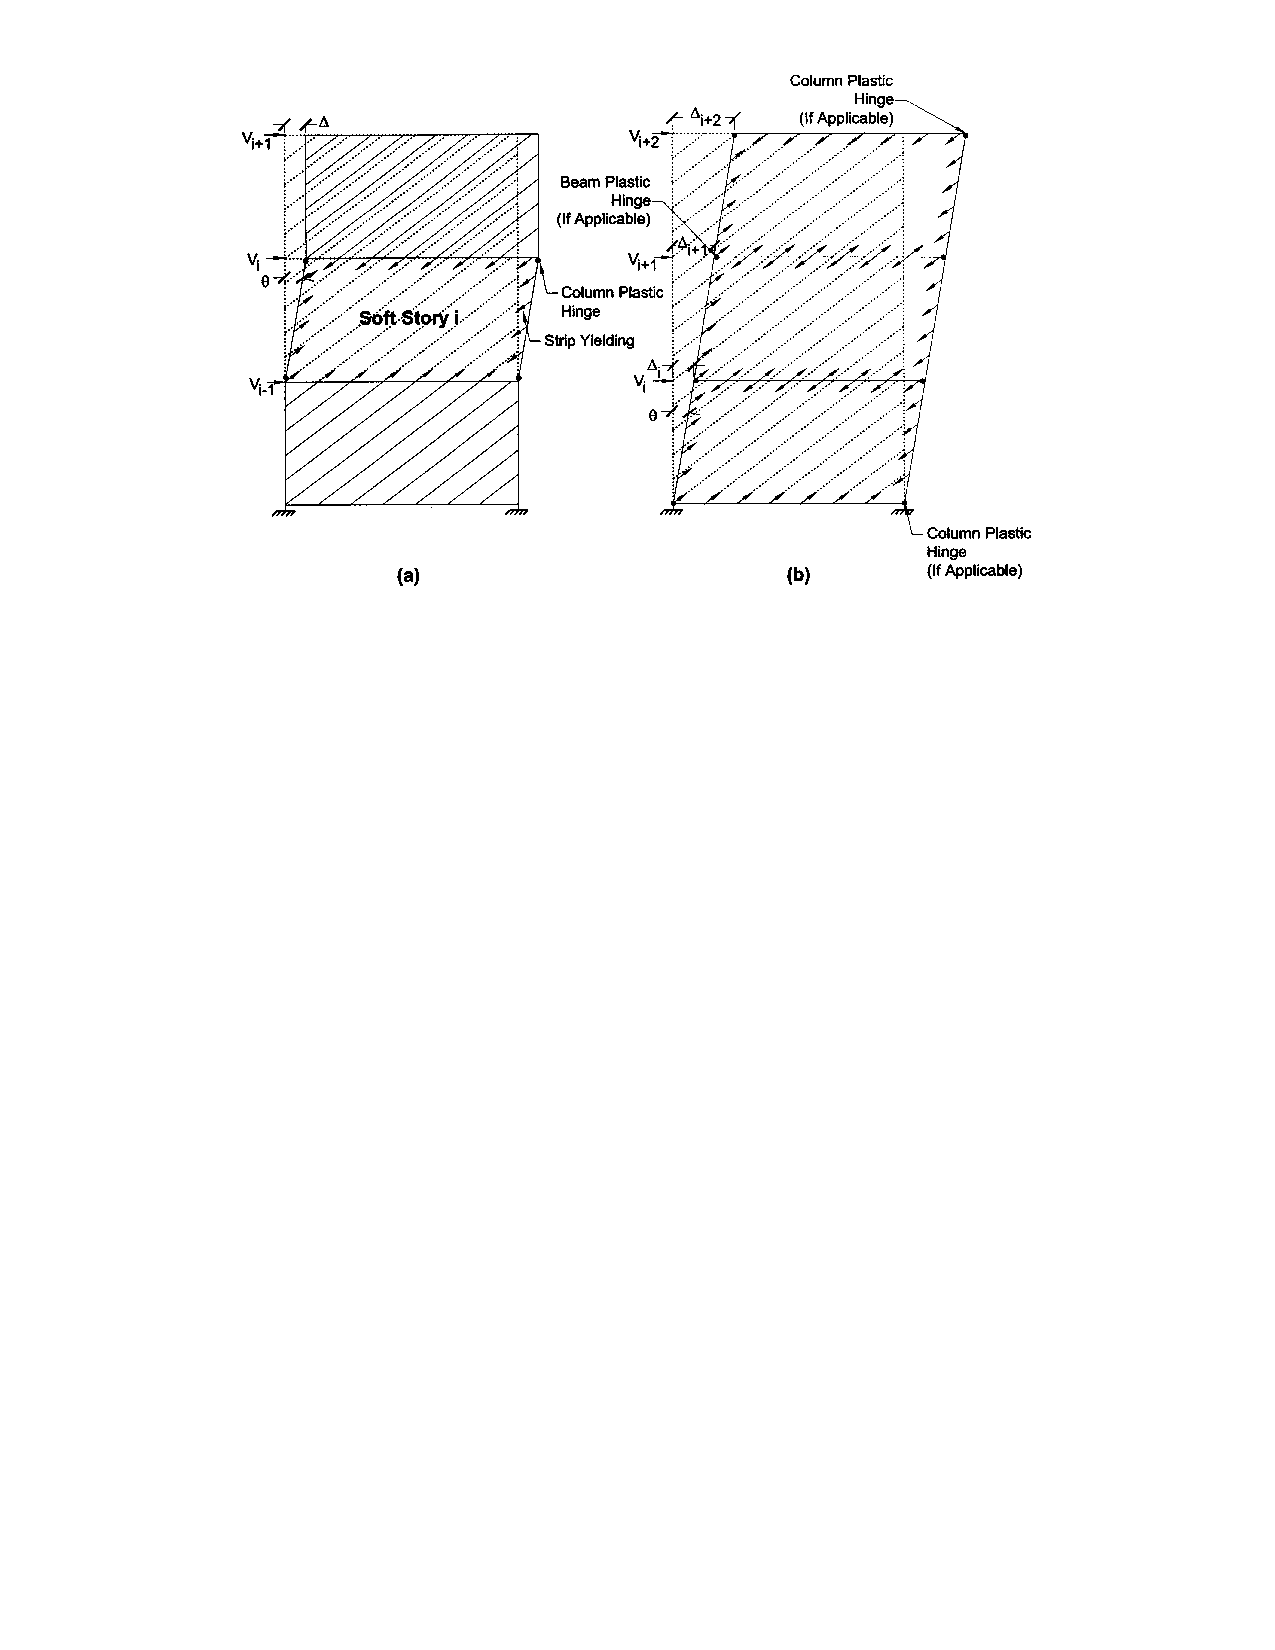
\includegraphics[width=12cm]{Berman2003.pdf}
  \bicaption{多层钢板剪力墙破坏模式}{Collapse mechanisms for multistory steel plate shear walls}
  \label{fig:Berman2003}
\end{figure}

在确定钢板剪力墙结构力学性能与设计方法时,较为关键的因素是拉力带倾角。\authornumcite{Thorburn1983}基于最小势能原理,提出了钢板剪力墙拉力带倾角计算公式:

\begin{equation}
\tan^4\alpha=\frac{1+\frac{Lw}{2A_{\rm{c}}}}{1+\frac{hw}{A_{\rm{b}}}}\qquad\mbox{(刚性边框柱)}
\label{Equ:1}
\end{equation}

\begin{equation}
\tan2\alpha=\frac{L}{H}\qquad\mbox{(柔性边框柱)}
\label{Equ:2}
\end{equation}

\authornumcite{Timler1983}考虑了边框柱有限刚度,对式~\ref{Equ:1}进行了修正:

\begin{equation}
\tan^4\alpha=\frac{1+\frac{Lw}{2A_{\rm{c}}}}{1+\left(\frac{1}{A_{\rm{b}}}+\frac{h^3}{360L_{\rm{c}}}\right)}
\label{Equ:3}
\end{equation}

\backmatter
% 参考文献
\printXAUATbibliography

% 附录
\begin{appendix}
    \chapter{公式推导一}
\section{section 1}
\section{section 2}

\chapter{公式推导二}
\section{section 1}
\section{section 2}

\end{appendix}

% 个人简历
\begin{resume}
    \resumeitem{个人简历:}
\noindent xxxx 年 xx 月 xx 日出生于 xx 省 xx 县。\\
\noindent xxxx 年 9 月考入 xx 大学 xx 系 xx 专业,xxxx 年 7 月本科毕业并获得 xx 学士学位。\\
\noindent xxxx 年 9 月免试进入 xx 大学 xx 系攻读 xx 学位至今。

\resumeitem{发表论文:} % 发表的和录用的合在一起
\begin{enumerate}[{[}1{]}]
\item Author. Title, Year,
  Volumn(Issue):Page. (SCI 收录, 检索号:$\times\times\times$.)

\end{enumerate}

\resumeitem{研究成果:} % 有就写,没有就删除
\begin{enumerate}[{[}1{]}]
\item 
\end{enumerate}

\end{resume}

% 致谢
\begin{acknowledgement}
    面对即将完稿的论文,心里感触良多。$\times\times\times$教授作为自己走上研究生科研之路上的领航者,教会了我独立思考的能力。$\times\times\times$老师严格的自律性、充分的执行力和认真的科研态度为我起到了标杆的作用。借此由衷的感谢$\times\times\times$老师一直以来......
\end{acknowledgement}

% 书脊
\shuji
\end{document}